% !TEX root =  ./main.tex

\section{Auxiliary Material}

\subsection{Auxiliary Material for the toy running example}

\begin{figure}[t]
\begin{minipage}{0.9\linewidth}
\footnotesize
\begin{verbatim}
myentities([cpowder,tpowder]).

myreactions([
    react([idle],[am],[am]),
    react([am],[idle],[am]),
    react([ccoin,cpowder],[nomilk],[cappuccino]),
    react([ccoin,cpowder,nomilk],[],[espresso]),
    react([tcoin,tpowder],[],[tea]),
    react([cpowder],[],[cpowder]),
    react([tpowder],[],[tpowder]),
    react([anger],[],[bang]) ]).

mycontext("[refill,student]").

myenvironment("[
    refill = ({nomilk}.refill 
            + {}.refill),
    student = (?{},{am},{tcoin}?.gettea 
             + ?{am},{},{ccoin}?.getcappuccino 
             + {idle}.student),
    gettea = (?{tea},{},{}?.student
            + ?{},{tea},{anger}?.student),
    getcappuccino = (?{cappuccino},{},{}?.student 
                    + ?{espresso},{},{anger}?.student) ]").
\end{verbatim}
\end{minipage}
\caption{\BioResolve implementation of the vending machine RS from \Cref{sec:student}.}
\label{fig:bioresolve:toy}
\end{figure}

\subsection{Auxiliary Material for the Comorbidity Treatment Case Study}

\subsection{Auxiliary Material for the Protein Signaling Networks Case Study}\label{app:psn}

\begin{figure}[t]
\begin{minipage}{0.9\linewidth}
\footnotesize
\begin{verbatim}
myentities([]).

myreactions([
    react([akt],[],[akt]),
    react([erbb3],[],[akt]),
    react([mtor],[],[akt]),
    react([pdk1],[],[akt]),
    react([erbb1],[e,p],[erbb1]),
    react([egf],[e,p],[erbb1]),
    react([plcg],[e,p],[erbb1]),
    react([erbb2],[e,t,p],[erbb2]),
    react([egf],[e,t,p],[erbb2]),
    react([erbb3],[e,t,p],[erbb2]),
    react([erbb3],[e,p],[erbb3]),
    react([hrg],[e,p],[erbb3]),
    react([erk12],[],[erk12]),
    react([egf],[],[erk12]),
    react([p],[],[erk12]),
    react([mek12],[],[erk12]),
    react([mek12],[],[mek12]),
    react([erbb1],[],[mek12]),
    react([erbb2],[],[mek12]),
    react([erbb3],[],[mek12]),
    react([mtor],[],[mtor]),
    react([p],[],[mtor]),
    react([akt],[],[mtor]),
    react([p70s6k],[],[p70s6k]),
    react([akt],[],[p70s6k]),
    react([mtor],[],[p70s6k]),
    react([erk12],[],[p70s6k]),
    react([pdk1],[],[pdk1]),
    react([erbb1],[],[pdk1]),
    react([erbb2],[],[pdk1]),
    react([erbb3],[],[pdk1]),
    react([mek12],[],[pdk1]),
    react([pkca],[],[pkca]),
    react([plcg],[],[pkca]),
    react([plcg],[],[plcg]),
    react([egf],[],[plcg]),
    react([erbb1],[],[plcg]),
    react([erbb2],[],[plcg]),
    react([erbb3],[],[plcg]) ]).

myenvironment("[
    k = {egf,hrg}.k,
    ket = {e,t}.ket,
    korep = ({e}.korep + {p}.korep),
    korept = ({e}.korept + {p}.korept + {t}.korept),
    kge = (?{erbb1},{},{e}?.kge 
          + ?{erbb2},{},{e}?.kge 
          + ?{},{erbb1,erbb2},{}?.kge) ]").

\end{verbatim}
\end{minipage}
\caption{\BioResolve implementation of the protein signaling network case study from \Cref{sec:ccReact}.}
\label{fig:bioresolve:psn}
\end{figure}

    


\subsection{Auxiliary Material for the T Cell Differentiation Case Study}

\begin{figure}[t]
	\begin{center}
		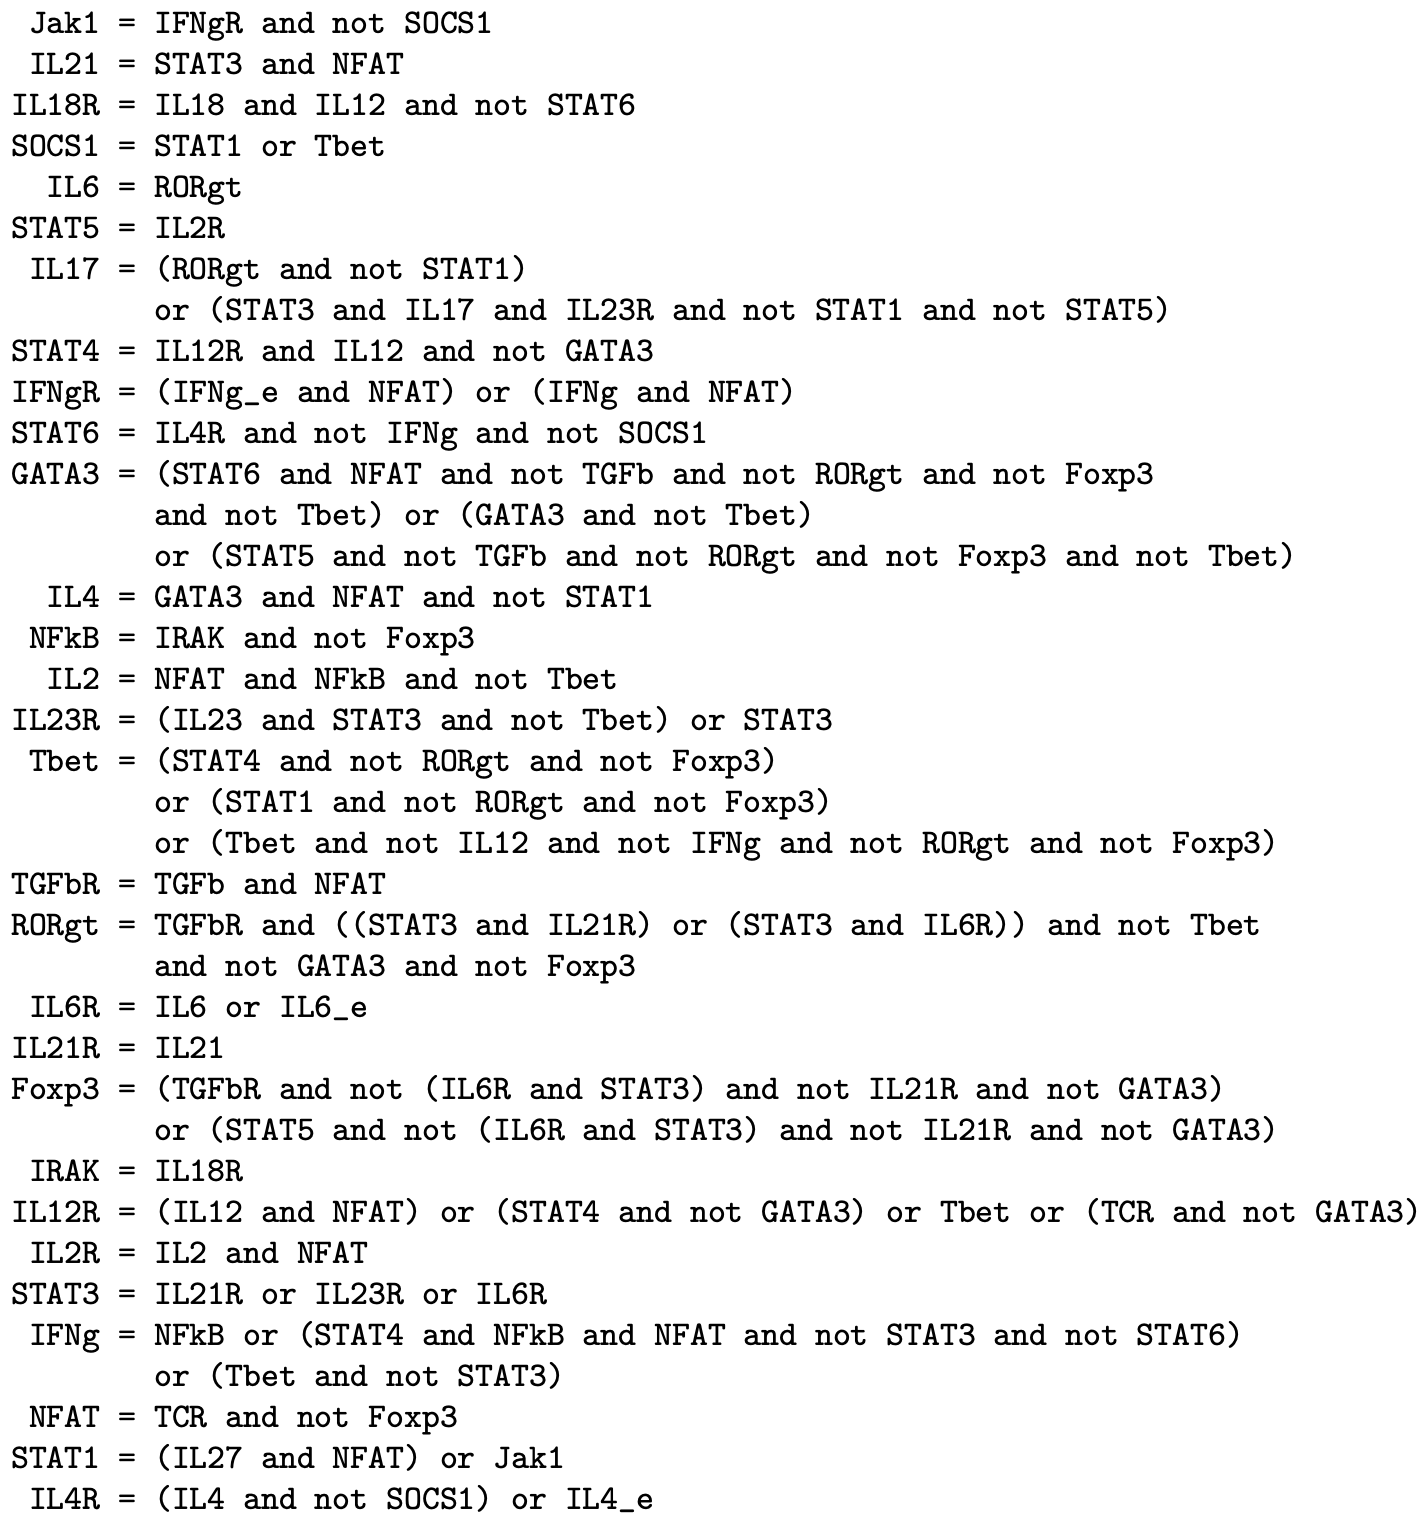
\includegraphics[width=0.49\textwidth]{figs-datamod2023/TcellBN.png}
	\end{center}
%\fontsize{8}{8}
%\begin{verbatim}
% Jak1 = IFNgR and not SOCS1 
% IL21 = STAT3 and NFAT
%IL18R = IL18 and IL12 and not STAT6 
%SOCS1 = STAT1 or Tbet 
%  IL6 = RORgt 
%STAT5 = IL2R 
% IL17 = (RORgt and not STAT1) 
%        or (STAT3 and IL17 and IL23R and not STAT1 and not STAT5) 
%STAT4 = IL12R and IL12 and not GATA3 
%IFNgR = (IFNg_e and NFAT) or (IFNg and NFAT) 
%STAT6 = IL4R and not IFNg and not SOCS1 
%GATA3 = (STAT6 and NFAT and not TGFb and not RORgt and not Foxp3 
%        and not Tbet) or (GATA3 and not Tbet) 
%        or (STAT5 and not TGFb and not RORgt and not Foxp3 and not Tbet) 
%  IL4 = GATA3 and NFAT and not STAT1 
% NFkB = IRAK and not Foxp3 
%  IL2 = NFAT and NFkB and not Tbet 
%IL23R = (IL23 and STAT3 and not Tbet) or STAT3 
% Tbet = (STAT4 and not RORgt and not Foxp3) 
%        or (STAT1 and not RORgt and not Foxp3) 
%        or (Tbet and not IL12 and not IFNg and not RORgt and not Foxp3) 
%TGFbR = TGFb and NFAT 
%RORgt = TGFbR and ((STAT3 and IL21R) or (STAT3 and IL6R)) and not Tbet 
%        and not GATA3 and not Foxp3 
% IL6R = IL6 or IL6_e 
%IL21R = IL21 
%Foxp3 = (TGFbR and not (IL6R and STAT3) and not IL21R and not GATA3) 
%        or (STAT5 and not (IL6R and STAT3) and not IL21R and not GATA3) 
% IRAK = IL18R 
%IL12R = (IL12 and NFAT) or (STAT4 and not GATA3) or Tbet or (TCR and not GATA3) 
% IL2R = IL2 and NFAT 
%STAT3 = IL21R or IL23R or IL6R 
% IFNg = NFkB or (STAT4 and NFkB and NFAT and not STAT3 and not STAT6) 
%        or (Tbet and not STAT3) 
% NFAT = TCR and not Foxp3 
%STAT1 = (IL27 and NFAT) or Jak1 
% IL4R = (IL4 and not SOCS1) or IL4_e 
%\end{verbatim}
	\caption{Boolean updates of the T Cell differentiation model from \cite{puniya2018mechanistic}, available at \cite{ModelCellCollective}.}
	\label{fig:boolean-formulas}
\end{figure}

\begin{figure}[t]
\begin{minipage}{0.9\linewidth}
\footnotesize
\begin{verbatim}
myreactions([
    react([stat5],[gata3,il21r,il6r],[foxp3]),
    react([stat5],[gata3,il21r,stat3],[foxp3]),
    react([tgfbr],[gata3,il21r,il6r],[foxp3]),
    react([tgfbr],[gata3,il21r,stat3],[foxp3]),
    react([gata3],[tbet],[gata3]),
    react([nfat,stat6],[foxp3,rorgt,tbet,tgfb],[gata3]),
    react([stat5],[foxp3,rorgt,tbet,tgfb],[gata3]),
    react([nfat,nfkb,stat4],[stat3,stat6],[ifng]),
    react([nfkb],[],[ifng]),
    react([tbet],[stat3],[ifng]),
    react([ifng,nfat],[],[ifngr]),
    react([ifnge,nfat],[],[ifngr]),
    react([il12,nfat],[],[il12r]),
    react([tbet],[],[il12r]),
    react([tcr],[gata3],[il12r]),
    react([il17,il23r,stat3],[stat1,stat5],[il17]),
    react([rorgt],[stat1],[il17]),
    react([il12,il18],[stat6],[il18r]),
    react([nfat,nfkb],[tbet],[il2]),
    react([nfat,stat3],[],[il21]),
    react([il21],[],[il21r]),
    react([il23,stat3],[tbet],[il23r]),
    react([stat3],[],[il23r]),
    react([il2,nfat],[],[il2r]),
    react([stat4],[gata3],[il2r]),
    react([gata3,nfat],[stat1],[il4]),
    react([il4],[socs1],[il4r]),
    react([il4e],[],[il4r]),
    react([rorgt],[],[il6]),
    react([il6],[],[il6r]),
    react([il6e],[],[il6r]),
    react([il18r],[],[irak]),
    react([ifngr],[socs1],[jak1]),
    react([tcr],[foxp3],[nfat]),
    react([irak],[foxp3],[nfkb]),
    react([il21r,stat3,tgfbr],[foxp3,gata3,tbet],[rorgt]),
    react([il6r,stat3,tgfbr],[foxp3,gata3,tbet],[rorgt]),
    react([stat1],[],[socs1]),
    react([tbet],[],[socs1]),
    react([il27,nfat],[],[stat1]),
    react([jak1],[],[stat1]),
    react([il21r],[],[stat3]),
    react([il23r],[],[stat3]),
    react([il6r],[],[stat3]),
    react([il12,il12r],[gata3],[stat4]),
    react([il2r],[],[stat5]),
    react([il4r],[ifng,socs1],[stat6]),
    react([stat1],[foxp3,rorgt],[tbet]),
    react([stat4],[foxp3,rorgt],[tbet]),
    react([tbet],[foxp3,ifng,il12,rorgt],[tbet]),
    react([nfat,tgfb],[],[tgfbr]) ]).
    
\end{verbatim}
\end{minipage}
\caption{\BioResolve implementation of the T cell case study from \Cref{sec:datamod2023}.}
\label{fig:bioresolve:tcell}
\end{figure}


